\hypertarget{a00004}{
\section{Dokumentacja klasy md5wrapper}
\label{d0/d0b/a00004}\index{md5wrapper@{md5wrapper}}
}
{\tt \#include $<$md5wrapper.h$>$}

Diagram współpracy dla md5wrapper:\nopagebreak
\begin{figure}[H]
\begin{center}
\leavevmode
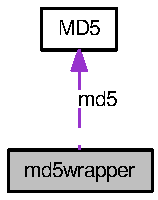
\includegraphics[width=112pt]{d4/d6d/a00055}
\end{center}
\end{figure}
\subsection*{Metody publiczne}
\begin{CompactItemize}
\item 
\hyperlink{a00004_ae8138b76b89d93a4c21077b76d57c07}{md5wrapper} ()
\item 
\hyperlink{a00004_65e78258ad508d83be81d395f8bd43f4}{$\sim$md5wrapper} ()
\item 
std::string \hyperlink{a00004_225ba5a78228b867c3f17fdba959d8e6}{getHashFromString} (std::string text)
\item 
std::string \hyperlink{a00004_e6cd2a7928b997c5d6388ae81a0d841a}{getHashFromFile} (std::string filename)
\end{CompactItemize}
\subsection*{Metody prywatne}
\begin{CompactItemize}
\item 
std::string \hyperlink{a00004_608ecf61c0ecdf2fcb772e9fd6c51d5f}{hashit} (std::string text)
\item 
std::string \hyperlink{a00004_74f856c53740d3beb133074baffd21aa}{convToString} (unsigned char $\ast$bytes)
\end{CompactItemize}
\subsection*{Atrybuty prywatne}
\begin{CompactItemize}
\item 
\hyperlink{a00002}{MD5} $\ast$ \hyperlink{a00004_fe675f7d8993ec64ddefa902dff431fa}{md5}
\end{CompactItemize}


\subsection{Opis szczegółowy}


Definicja w linii 23 pliku md5wrapper.h.

\subsection{Dokumentacja konstruktora i destruktora}
\hypertarget{a00004_ae8138b76b89d93a4c21077b76d57c07}{
\index{md5wrapper@{md5wrapper}!md5wrapper@{md5wrapper}}
\index{md5wrapper@{md5wrapper}!md5wrapper@{md5wrapper}}
\subsubsection[{md5wrapper}]{\setlength{\rightskip}{0pt plus 5cm}md5wrapper::md5wrapper ()}}
\label{d0/d0b/a00004_ae8138b76b89d93a4c21077b76d57c07}




Definicja w linii 70 pliku md5wrapper.cpp.\hypertarget{a00004_65e78258ad508d83be81d395f8bd43f4}{
\index{md5wrapper@{md5wrapper}!$\sim$md5wrapper@{$\sim$md5wrapper}}
\index{$\sim$md5wrapper@{$\sim$md5wrapper}!md5wrapper@{md5wrapper}}
\subsubsection[{$\sim$md5wrapper}]{\setlength{\rightskip}{0pt plus 5cm}md5wrapper::$\sim$md5wrapper ()}}
\label{d0/d0b/a00004_65e78258ad508d83be81d395f8bd43f4}




Definicja w linii 77 pliku md5wrapper.cpp.

\subsection{Dokumentacja funkcji składowych}
\hypertarget{a00004_74f856c53740d3beb133074baffd21aa}{
\index{md5wrapper@{md5wrapper}!convToString@{convToString}}
\index{convToString@{convToString}!md5wrapper@{md5wrapper}}
\subsubsection[{convToString}]{\setlength{\rightskip}{0pt plus 5cm}std::string md5wrapper::convToString (unsigned char $\ast$ {\em bytes})\hspace{0.3cm}{\tt  \mbox{[}private\mbox{]}}}}
\label{d0/d0b/a00004_74f856c53740d3beb133074baffd21aa}




Definicja w linii 53 pliku md5wrapper.cpp.

Here is the caller graph for this function:\nopagebreak
\begin{figure}[H]
\begin{center}
\leavevmode
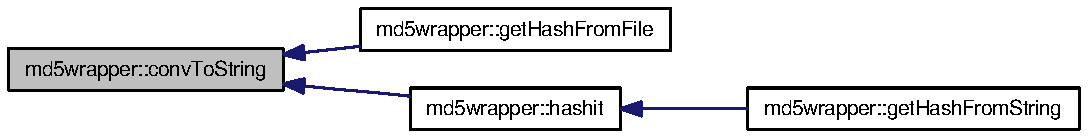
\includegraphics[width=279pt]{d0/d0b/a00004_74f856c53740d3beb133074baffd21aa_icgraph}
\end{center}
\end{figure}
\hypertarget{a00004_e6cd2a7928b997c5d6388ae81a0d841a}{
\index{md5wrapper@{md5wrapper}!getHashFromFile@{getHashFromFile}}
\index{getHashFromFile@{getHashFromFile}!md5wrapper@{md5wrapper}}
\subsubsection[{getHashFromFile}]{\setlength{\rightskip}{0pt plus 5cm}std::string md5wrapper::getHashFromFile (std::string {\em filename})}}
\label{d0/d0b/a00004_e6cd2a7928b997c5d6388ae81a0d841a}




Definicja w linii 100 pliku md5wrapper.cpp.

Oto graf wywołań dla tej funkcji:\nopagebreak
\begin{figure}[H]
\begin{center}
\leavevmode
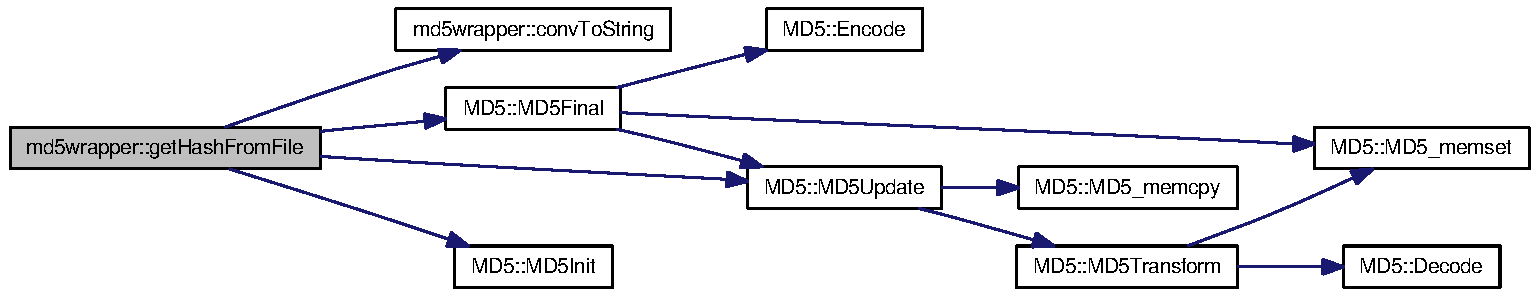
\includegraphics[width=387pt]{d0/d0b/a00004_e6cd2a7928b997c5d6388ae81a0d841a_cgraph}
\end{center}
\end{figure}
\hypertarget{a00004_225ba5a78228b867c3f17fdba959d8e6}{
\index{md5wrapper@{md5wrapper}!getHashFromString@{getHashFromString}}
\index{getHashFromString@{getHashFromString}!md5wrapper@{md5wrapper}}
\subsubsection[{getHashFromString}]{\setlength{\rightskip}{0pt plus 5cm}std::string md5wrapper::getHashFromString (std::string {\em text})}}
\label{d0/d0b/a00004_225ba5a78228b867c3f17fdba959d8e6}




Definicja w linii 87 pliku md5wrapper.cpp.

Oto graf wywołań dla tej funkcji:\nopagebreak
\begin{figure}[H]
\begin{center}
\leavevmode
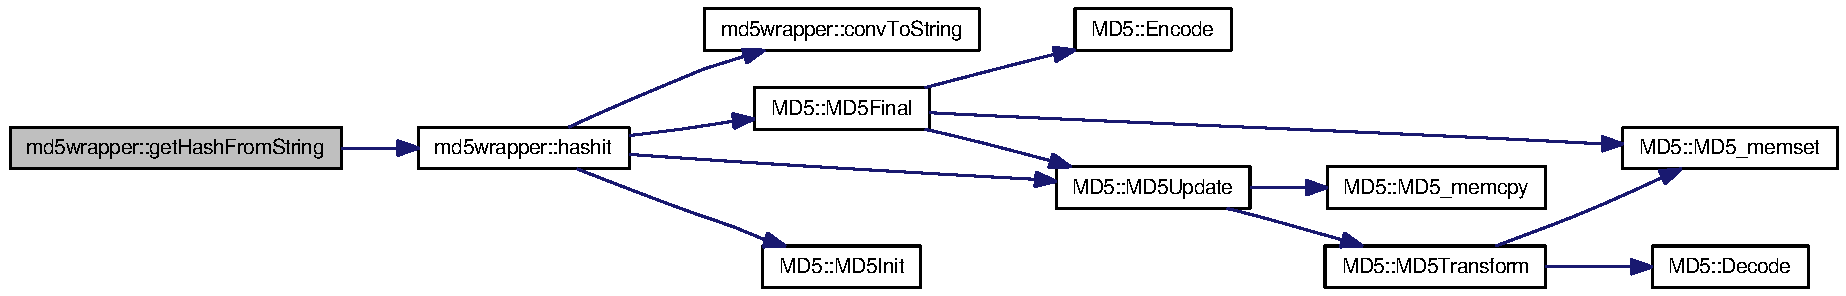
\includegraphics[width=420pt]{d0/d0b/a00004_225ba5a78228b867c3f17fdba959d8e6_cgraph}
\end{center}
\end{figure}
\hypertarget{a00004_608ecf61c0ecdf2fcb772e9fd6c51d5f}{
\index{md5wrapper@{md5wrapper}!hashit@{hashit}}
\index{hashit@{hashit}!md5wrapper@{md5wrapper}}
\subsubsection[{hashit}]{\setlength{\rightskip}{0pt plus 5cm}std::string md5wrapper::hashit (std::string {\em text})\hspace{0.3cm}{\tt  \mbox{[}private\mbox{]}}}}
\label{d0/d0b/a00004_608ecf61c0ecdf2fcb772e9fd6c51d5f}




Definicja w linii 28 pliku md5wrapper.cpp.

Oto graf wywołań dla tej funkcji:\nopagebreak
\begin{figure}[H]
\begin{center}
\leavevmode
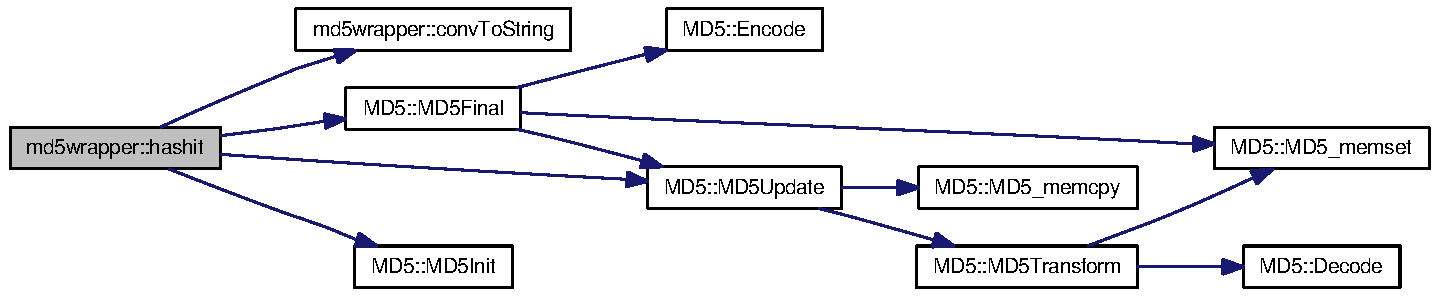
\includegraphics[width=363pt]{d0/d0b/a00004_608ecf61c0ecdf2fcb772e9fd6c51d5f_cgraph}
\end{center}
\end{figure}


Here is the caller graph for this function:\nopagebreak
\begin{figure}[H]
\begin{center}
\leavevmode
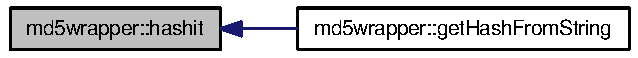
\includegraphics[width=171pt]{d0/d0b/a00004_608ecf61c0ecdf2fcb772e9fd6c51d5f_icgraph}
\end{center}
\end{figure}


\subsection{Dokumentacja atrybutów składowych}
\hypertarget{a00004_fe675f7d8993ec64ddefa902dff431fa}{
\index{md5wrapper@{md5wrapper}!md5@{md5}}
\index{md5@{md5}!md5wrapper@{md5wrapper}}
\subsubsection[{md5}]{\setlength{\rightskip}{0pt plus 5cm}{\bf MD5}$\ast$ {\bf md5wrapper::md5}\hspace{0.3cm}{\tt  \mbox{[}private\mbox{]}}}}
\label{d0/d0b/a00004_fe675f7d8993ec64ddefa902dff431fa}




Definicja w linii 26 pliku md5wrapper.h.

Dokumentacja dla tej klasy została wygenerowana z plików:\begin{CompactItemize}
\item 
\hyperlink{a00013}{md5wrapper.h}\item 
\hyperlink{a00012}{md5wrapper.cpp}\end{CompactItemize}
